\section{Lineares Hashing 1}

Gegeben ist die unten skizzierte lineare Hashtabelle mit $q = 5$ Buckets, die jeweils eine Größe $b = 2$ besitzen. Es wurden bisher die 4 vorgegebenen Schlüssel in die Tabelle eingefügt und noch keine Verdopplungen ausgeführt. Positionszeiger $p = 0$. Die Folge von Hashfunktionen sei $h_{j}(k) = k \bmod(2^{j} \cdot q), \; j = 0,1,$ \ldots

Fügen Sie die folgenden Schlüssel in der angegebenen Reihenfolge in die Tabelle ein. Verwenden Sie dabei kontrolliertes Splitting mit Schwellenwert $\alpha = 0,8$. \\
18, 50, 66, 2, 35, 51, 17, 22, 38, 85, 32, 16, 59, 9

\begin{minipage}{5cm}
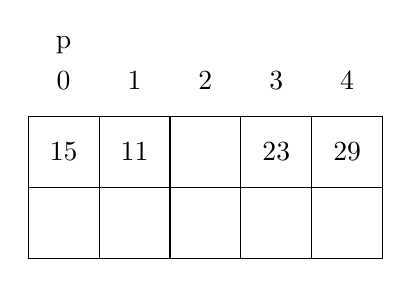
\begin{tikzpicture}
	\draw[step=.9cm] (0, 0) grid +(4.5, 1.8);
	\node at (0.45, 1.35) {15};
	\node at (1.35, 1.35) {11};
	\node at (3.15, 1.35) {23};
	\node at (4.05, 1.35) {29};
	\node at (0.45, 2.7) {p};
	\node at (0.45, 2.25) {0};
	\node at (1.35, 2.25) {1};
	\node at (2.25, 2.25) {2};
	\node at (3.15, 2.25) {3};
	\node at (4.05, 2.25) {4};
\end{tikzpicture}
\end{minipage} \hfill
\begin{minipage}{0.65\textwidth}
Belegungsfaktor:
\[\beta = \frac{N}{ (q \cdot 2^{L} + p) \cdot b} = \frac{4}{(5 \cdot 2^{0} + 0) \cdot 2} = 0,4\]
mit L Anzahl der schon vollständig durchgeführten Verdoppelungen
\end{minipage}


\begin{beamerText}
\pagebreak
\begin{Form}
Schwellenwert $\alpha = 0,8$. \\
18, 50, 66, 2, 35, 51, 17, 22, 38, 85, 32, 16, 59, 9

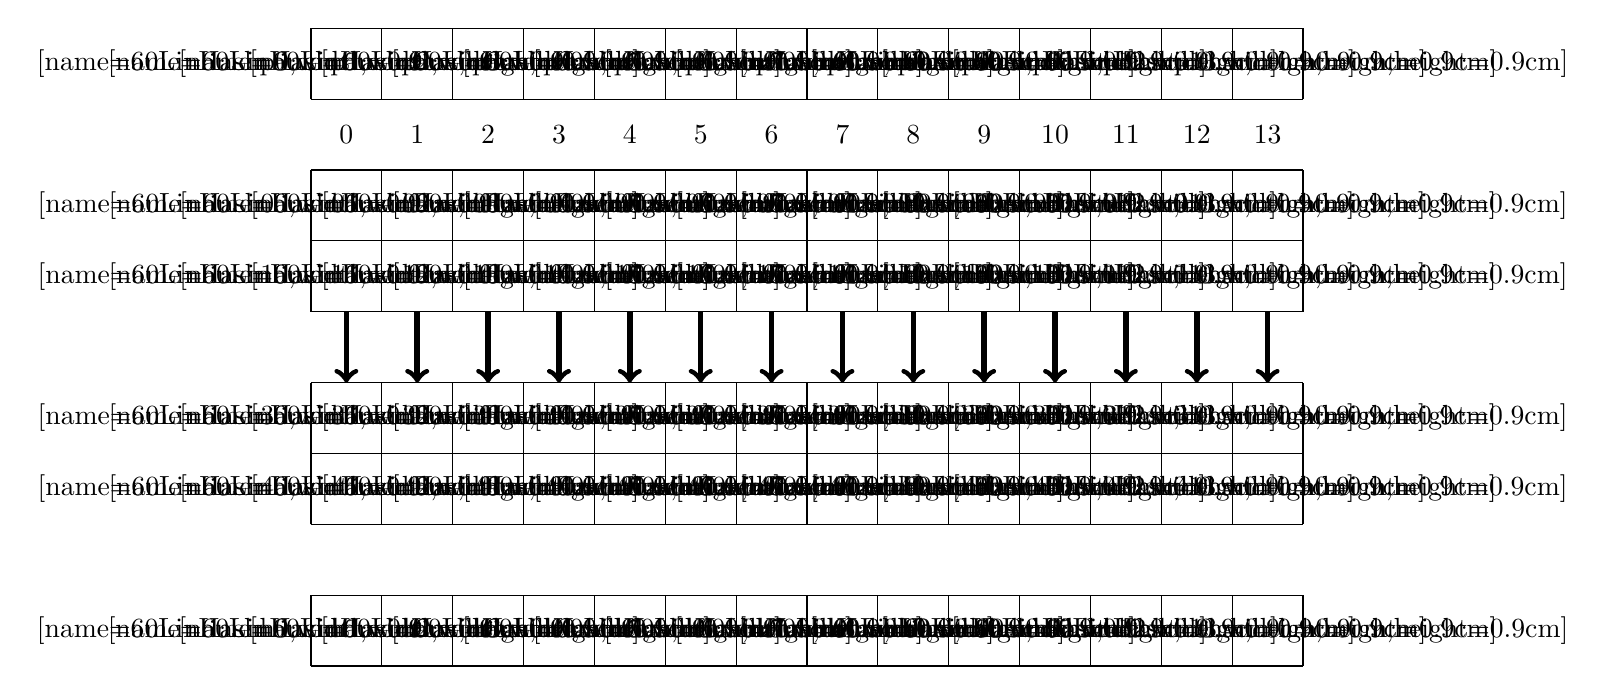
\begin{tikzpicture}
	\def\size{13}
	%template
	\draw[step=.9cm] (0, 5.4) grid +(0.9+\size*0.9, -0.9001);
%	\draw (0, 4.5) -- (0.9+\size*0.9, 4.5);

	\draw[step=.9cm] (0, 3.6) grid +(0.9+\size*0.9, -1.8001);
%	\draw (0, 1.8) -- (0.9+\size*0.9, 1.8);

	\draw[step=.9cm] (0, 0.9) grid +(0.9+\size*0.9, -1.8001);
%	\draw (0, -0.9) -- (0.9+\size*0.9, -0.9);

	\draw[step=.9cm] (0, -2.7) grid +(0.9+\size*0.9, 0.9);

	\foreach \j in {0,1,3,4}
	\foreach \i in {0,...,\size}
	{
		\node at (0.35+0.9*\i, 3.15-0.9*\j) {\TextField[name=60LinHash\j\i,width=0.9cm,height=0.9cm]{\null}};
	}
	\foreach \i in {0,...,\size}{
		% Textfield für P
		\node at (0.35+0.9*\i, 3.15-0.9*-2) {\TextField[name=60LinHashp\i,width=0.9cm,height=0.9cm]{\null}};
		%index
		\node at (0.45+0.9*\i, 4.05) {\i};
		% Verbindung zum Overflow bucket
		\draw [<-, line width=2pt] (0.45+0.9*\i, 0.9) -- (0.45+0.9*\i, 1.8);
		% Textfield für h_1 und h_2
		\node at (0.35+0.9*\i, -2.25) {\TextField[name=60LinHashh\i,width=0.9cm,height=0.9cm]{\null}};
	}

\end{tikzpicture}

\PushButton[onclick={
for(i=0; i< 14; i++) {
	this.getField("60LinHashp" + i.toString()).value='';
	this.getField("60LinHash0" + i.toString()).value='';
	this.getField("60LinHash1" + i.toString()).value='';
	this.getField("60LinHash3" + i.toString()).value='';
	this.getField("60LinHash4" + i.toString()).value='';
	this.getField("60LinHashh" + i.toString()).value='';
}
	this.getField("60LinHashp0").value="p";
	this.getField("60LinHash00").value=15;
	this.getField("60LinHash01").value=11;
	this.getField("60LinHash03").value=23;
	this.getField("60LinHash04").value=29;
	this.getField("60LinHashp5").value="X";
	this.getField("60LinHashh0").value="h0";
	this.getField("60LinHashh1").value="h0";
	this.getField("60LinHashh2").value="h0";
	this.getField("60LinHashh3").value="h0";
	this.getField("60LinHashh4").value="h0";
	this.getField("60LinHashN").value="4";
	this.getField("60LinHashL").value="0";
	this.getField("60LinHashP").value="0";
	this.getField("60LinHashOut").value='';
}]{Init}
\PushButton[onclick={
	var n = parseInt(this.getField("60LinHashN").value);
	var p = parseInt(this.getField("60LinHashP").value);
	var l = parseInt(this.getField("60LinHashL").value);
	this.getField("60LinHashOut").value = n/((5*Math.pow(2,l)+p)*2);
}]{Calculate}
\begin{align*}
\beta = \frac{N}{ (q \cdot 2^{L} + p) \cdot b} = \frac{\TextField[name=60LinHashN,width=0.9cm,height=0.9cm]{\null}}{(5 \cdot 2^{\TextField[name=60LinHashL,width=0.9cm,height=0.9cm]{\null}} + \TextField[name=60LinHashP,width=0.9cm,height=0.9cm]{\null}) \cdot 2} = \TextField[name=60LinHashOut, width=2cm, height=0.9cm]{\null} \leq 0.8
\end{align*}
\end{Form}
\end{beamerText}

\begin{solution}
Folgende Hashfunktionen kommen zum Einsatz:
\begin{itemize}
	\item $h_{0}(k) = k \bmod (2^0 \cdot 5) = k \bmod 5$
	\item $h_{1}(k) = k \bmod (2^1 \cdot 5) = k \bmod 10$
	\item $h_{2}(k) = k \bmod (2^2 \cdot 5) = k \bmod 20$
\end{itemize}
%1
\begin{minipage}{0.4\textwidth}
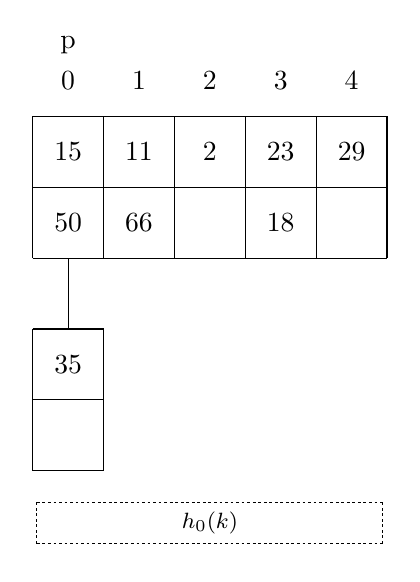
\begin{tikzpicture}
	%template
	\draw[step=.9cm] (0, -0.9) grid +(0.9, 1.8);
	\draw[step=.9cm] (0, 1.8) grid +(4.5, 1.8);
	\draw (0, 1.8) -- (4.5, 1.8);
	\draw (0.45, 0.9) -- (0.45, 1.8);
	\draw (0, -0.9) -- (0.9, -0.9);
	%index
	\node at (0.45, 4.5) {p};
	\node at (0.45, 4.05) {0};
	\node at (1.35, 4.05) {1};
	\node at (2.25, 4.05) {2};
	\node at (3.15, 4.05) {3};
	\node at (4.05, 4.05) {4};
	%inserted keys
	\node at (0.45, 3.15) {15};
	\node at (0.45, 2.25) {50};
	\node at (0.45, 0.45) {35};
	\node at (1.35, 3.15) {11};
	\node at (1.35, 2.25) {66};
	\node at (2.25, 3.15) {2};
	\node at (3.15, 3.15) {23};
	\node at (3.15, 2.25) {18};
	\node at (4.05, 3.15) {29};
	%hash functions
	\node at (2.25, -1.55) {\dashbox{1}(125,15){\footnotesize $h_0(k)$}};
\end{tikzpicture}
\end{minipage}
\begin{minipage}{0.55\textwidth}
Einfügen der Schlüssel 18, 50, 66, 2 und 35 lässt $\beta > \alpha$ werden: \\
\[\beta = \frac{N}{ (q \cdot 2^{L} + p) \cdot b} = \frac{9}{(5 \cdot 2^{0} + 0) \cdot 2} = \textcolor{red}{0,9}\]
\end{minipage}

%2
\begin{minipage}{0.4\textwidth}
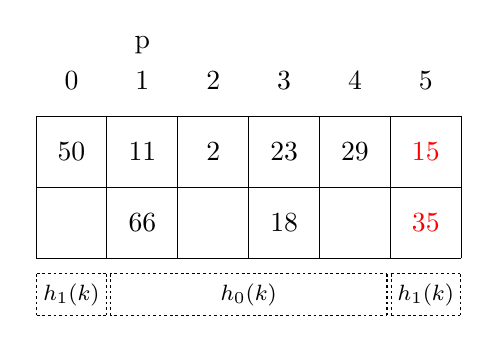
\begin{tikzpicture}
	%template
	\draw[step=.9cm] (0, 0) grid +(5.4, 1.8);
	\draw (0, 0) -- (5.4, 0);
	%index
	\node at (1.35, 2.7) {p};
	\node at (0.45, 2.25) {0};
	\node at (1.35, 2.25) {1};
	\node at (2.25, 2.25) {2};
	\node at (3.15, 2.25) {3};
	\node at (4.05, 2.25) {4};
	\node at (4.95, 2.25) {5};
	%inserted keys
	\node at (0.45, 1.35) {50};
	\node at (1.35, 1.35) {11};
	\node at (1.35, 0.45) {66};
	\node at (2.25, 1.35) {2};
	\node at (3.15, 1.35) {23};
	\node at (3.15, 0.45) {18};
	\node at (4.05, 1.35) {29};
	\node at (4.95, 1.35)  {\textcolor{red}{15}};
	\node at (4.95, 0.45) {\textcolor{red}{35}};
	%hash functions
	\node at (2.7, -0.45) {\dashbox{1}(100,15){\footnotesize $h_0(k)$}};
	\node at (4.95, -0.45) {\dashbox{1}(25,15){\footnotesize $h_1(k)$}};
	\node at (0.45, -0.45) {\dashbox{1}(25,15){\footnotesize $h_1(k)$}};
\end{tikzpicture}
\end{minipage}
\begin{minipage}{0.55\textwidth}
Splitt von Bucket 0, es werden jetzt $h_0(k)$ und $h_1(k)$ angewendet. \\
\[\beta = \frac{N}{ (q \cdot 2^{L} + p) \cdot b} = \frac{9}{(5 \cdot 2^{0} + 1) \cdot 2} = 0,75\]
\end{minipage}

%3
\begin{minipage}{0.4\textwidth}
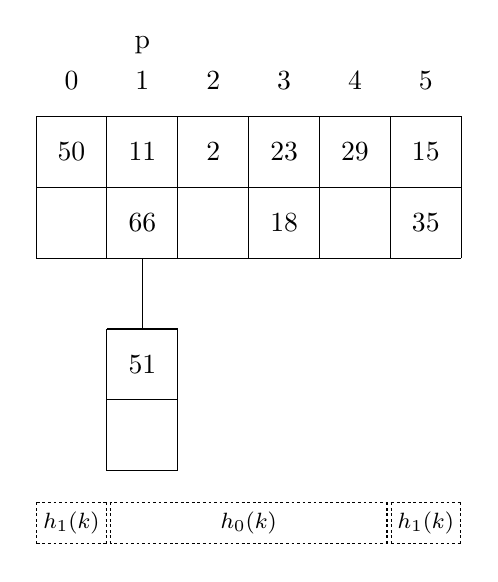
\begin{tikzpicture}
	%template
	\draw[step=.9cm] (0.9, -0.9) grid +(0.9, 1.8);
	\draw[step=.9cm] (0, 1.8) grid +(5.4, 1.8);
	\draw (0, 1.8) -- (5.4, 1.8);
	\draw (1.35, 0.9) -- (1.35, 1.8);
	\draw (0.9, -0.9) -- (1.8, -0.9);
	%index
	\node at (1.35, 4.5) {p};
	\node at (0.45, 4.05) {0};
	\node at (1.35, 4.05) {1};
	\node at (2.25, 4.05) {2};
	\node at (3.15, 4.05) {3};
	\node at (4.05, 4.05) {4};
	\node at (4.95, 4.05) {5};
	%inserted keys
	\node at (0.45, 3.15) {50};
	\node at (1.35, 3.15) {11};
	\node at (1.35, 2.25) {66};
	\node at (1.35, 0.45) {51};
	\node at (2.25, 3.15) {2};
	\node at (3.15, 3.15) {23};
	\node at (3.15, 2.25) {18};
	\node at (4.05, 3.15) {29};
	\node at (4.95, 3.15) {15};
	\node at (4.95, 2.25) {35};
	%hash functions
	\node at (2.7, -1.55) {\dashbox{1}(100,15){\footnotesize $h_0(k)$}};
	\node at (4.95, -1.55) {\dashbox{1}(25,15){\footnotesize $h_1(k)$}};
	\node at (0.45, -1.55) {\dashbox{1}(25,15){\footnotesize $h_1(k)$}};
\end{tikzpicture}
\end{minipage}
\begin{minipage}{0.55\textwidth}
Einfügen des Schlüssels 51 lässt $\beta > \alpha$ werden: \\
\[\beta = \frac{N}{ (q \cdot 2^{L} + p) \cdot b} = \frac{10}{(5 \cdot 2^{0} + 1) \cdot 2} = \textcolor{red}{0,83}\]
\end{minipage}

%4
\begin{minipage}{0.5\textwidth}
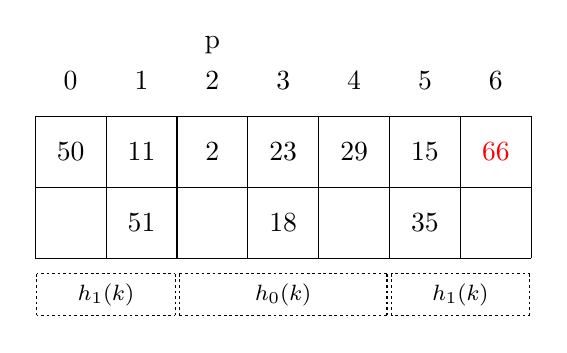
\begin{tikzpicture}
	%template
	\draw[step=.9cm] (0, 0) grid +(6.3, 1.8);
	\draw (0, 0) -- (6.3, 0);
	%index
	\node at (2.25, 2.7) {p};
	\node at (0.45, 2.25) {0};
	\node at (1.35, 2.25) {1};
	\node at (2.25, 2.25) {2};
	\node at (3.15, 2.25) {3};
	\node at (4.05, 2.25) {4};
	\node at (4.95, 2.25) {5};
	\node at (5.85, 2.25) {6};
	%inserted keys
	\node at (0.45, 1.35) {50};
	\node at (1.35, 1.35) {11};
	\node at (1.35, 0.45) {51};
	\node at (2.25, 1.35) {2};
	\node at (3.15, 1.35) {23};
	\node at (3.15, 0.45) {18};
	\node at (4.05, 1.35) {29};
	\node at (4.95, 1.35)  {15};
	\node at (4.95, 0.45) {35};
	\node at (5.85, 1.35) {\textcolor{red}{66}};
	%hash functions
	\node at (0.9, -0.45) {\dashbox{1}(50,15){\footnotesize $h_1(k)$}};
	\node at (3.15, -0.45) {\dashbox{1}(75,15){\footnotesize $h_0(k)$}};
	\node at (5.4, -0.45) {\dashbox{1}(50,15){\footnotesize $h_1(k)$}};
\end{tikzpicture}
\end{minipage}
\begin{minipage}{0.4\textwidth}
Splitt von Bucket 1 \\
\[\beta = \frac{N}{ (q \cdot 2^{L} + p) \cdot b} = \frac{10}{(5 \cdot 2^{0} + 2) \cdot 2} \] \[\beta = 0,71\]
\end{minipage}

%5
\begin{minipage}{0.5\textwidth}
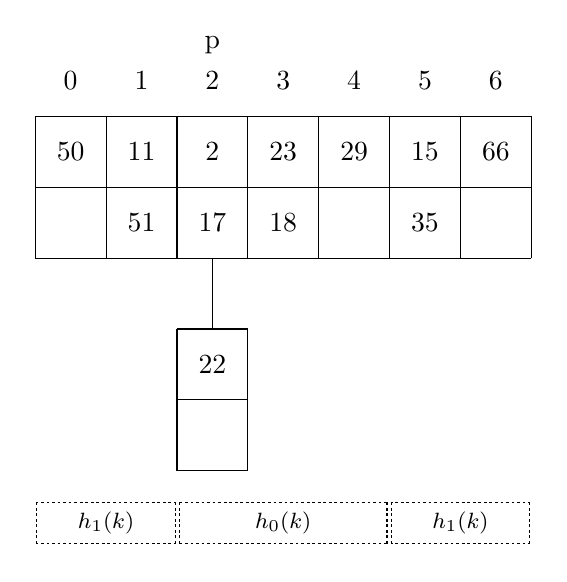
\begin{tikzpicture}
	%template
	\draw[step=.9cm] (1.8, -0.9) grid +(0.9, 1.8);
	\draw[step=.9cm] (0, 1.8) grid +(6.3, 1.8);
	\draw (0, 1.8) -- (6.3, 1.8);
	\draw (1.8, -0.9) -- (1.8, 0.9);
	\draw (2.25, 0.9) -- (2.25, 1.8);
	\draw (1.8, -0.9) -- (2.7, -0.9);
	%index
	\node at (2.25, 4.5) {p};
	\node at (0.45, 4.05) {0};
	\node at (1.35, 4.05) {1};
	\node at (2.25, 4.05) {2};
	\node at (3.15, 4.05) {3};
	\node at (4.05, 4.05) {4};
	\node at (4.95, 4.05) {5};
	\node at (5.85, 4.05) {6};
	%inserted keys
	\node at (0.45, 3.15) {50};
	\node at (1.35, 3.15) {11};
	\node at (1.35, 2.25) {51};
	\node at (2.25, 3.15) {2};
	\node at (2.25, 2.25) {17};
	\node at (2.25, 0.45) {22};
	\node at (3.15, 3.15) {23};
	\node at (3.15, 2.25) {18};
	\node at (4.05, 3.15) {29};
	\node at (4.95, 3.15) {15};
	\node at (4.95, 2.25) {35};
	\node at (5.85, 3.15) {66};
	%hash functions
	\node at (0.9, -1.55) {\dashbox{1}(50,15){\footnotesize $h_1(k)$}};
	\node at (3.15, -1.55) {\dashbox{1}(75,15){\footnotesize $h_0(k)$}};
	\node at (5.4, -1.55) {\dashbox{1}(50,15){\footnotesize $h_1(k)$}};
\end{tikzpicture}
\end{minipage}
\begin{minipage}{0.4\textwidth}
Einfügen der Schlüssel 17 und 22 lässt $\beta > \alpha$ werden: \\
\[\beta = \frac{N}{ (q \cdot 2^{L} + p) \cdot b} = \frac{12}{(5 \cdot 2^{0} + 2) \cdot 2}\] \[\beta = \textcolor{red}{0,86}\]
\end{minipage}

%6
Splitt von Bucket 2:

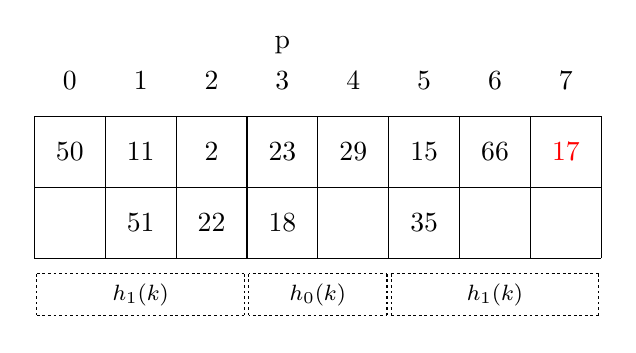
\begin{tikzpicture}
	%template
	\draw[step=.9cm] (0, 0) grid +(7.2, 1.8);
	\draw (0, 0) -- (7.2, 0);
	%index
	\node at (3.15, 2.7) {p};
	\node at (0.45, 2.25) {0};
	\node at (1.35, 2.25) {1};
	\node at (2.25, 2.25) {2};
	\node at (3.15, 2.25) {3};
	\node at (4.05, 2.25) {4};
	\node at (4.95, 2.25) {5};
	\node at (5.85, 2.25) {6};
	\node at (6.75, 2.25) {7};
	%inserted keys
	\node at (0.45, 1.35) {50};
	\node at (1.35, 1.35) {11};
	\node at (1.35, 0.45) {51};
	\node at (2.25, 1.35) {2};
	\node at (2.25, 0.45) {22};
	\node at (3.15, 1.35) {23};
	\node at (3.15, 0.45) {18};
	\node at (4.05, 1.35) {29};
	\node at (4.95, 1.35)  {15};
	\node at (4.95, 0.45) {35};
	\node at (5.85, 1.35) {66};
	\node at (6.75, 1.35) {\textcolor{red}{17}};
	%hash functions
	\node at (1.35, -0.45) {\dashbox{1}(75,15){\footnotesize $h_1(k)$}};
	\node at (3.6, -0.45) {\dashbox{1}(50,15){\footnotesize $h_0(k)$}};
	\node at (5.85, -0.45) {\dashbox{1}(75,15){\footnotesize $h_1(k)$}};
\end{tikzpicture}

\[\beta = \frac{N}{ (q \cdot 2^{L} + p) \cdot b} = \frac{12}{(5 \cdot 2^{0} + 3) \cdot 2} = 0,75\]

%7
Einfügen des Schlüssels 38 lässt $\beta > \alpha$ werden:

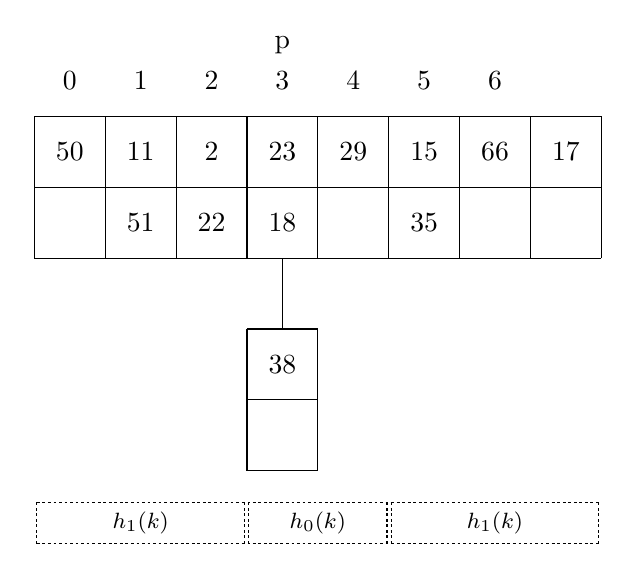
\begin{tikzpicture}
	%template
	\draw[step=.9cm] (2.7, -0.9) grid +(0.9, 1.8);
	\draw[step=.9cm] (0, 1.8) grid +(7.2, 1.8);
	\draw (0, 1.8) -- (7.2, 1.8);
	\draw (2.7, -0.9) -- (2.7, 0.9);
	\draw (3.15, 0.9) -- (3.15, 1.8);
	\draw (2.7, -0.9) -- (3.6, -0.9);
	%index
	\node at (3.15, 4.5) {p};
	\node at (0.45, 4.05) {0};
	\node at (1.35, 4.05) {1};
	\node at (2.25, 4.05) {2};
	\node at (3.15, 4.05) {3};
	\node at (4.05, 4.05) {4};
	\node at (4.95, 4.05) {5};
	\node at (5.85, 4.05) {6};
	%inserted keys
	\node at (0.45, 3.15) {50};
	\node at (1.35, 3.15) {11};
	\node at (1.35, 2.25) {51};
	\node at (2.25, 3.15) {2};
	\node at (2.25, 2.25) {22};
	\node at (3.15, 0.45) {38};
	\node at (3.15, 3.15) {23};
	\node at (3.15, 2.25) {18};
	\node at (4.05, 3.15) {29};
	\node at (4.95, 3.15) {15};
	\node at (4.95, 2.25) {35};
	\node at (5.85, 3.15) {66};
	\node at (6.75, 3.15) {17};
	%hash functions
	\node at (1.35, -1.55) {\dashbox{1}(75,15){\footnotesize $h_1(k)$}};
	\node at (3.6, -1.55) {\dashbox{1}(50,15){\footnotesize $h_0(k)$}};
	\node at (5.85, -1.55) {\dashbox{1}(75,15){\footnotesize $h_1(k)$}};
\end{tikzpicture}

\[\beta = \frac{N}{ (q \cdot 2^{L} + p) \cdot b} = \frac{13}{(5 \cdot 2^{0} + 3) \cdot 2} = \textcolor{red}{0,81}\]

%8
Splitt von Bucket 3:

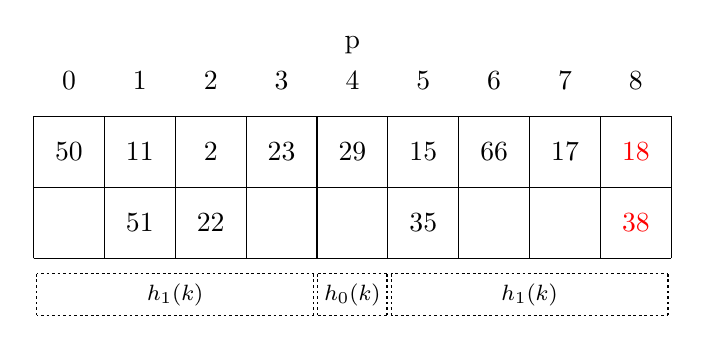
\begin{tikzpicture}
	%template
	\draw[step=.9cm] (0, 0) grid +(8.1, 1.8);
	\draw (0, 0) -- (8.1, 0);
	%index
	\node at (4.05, 2.7) {p};
	\node at (0.45, 2.25) {0};
	\node at (1.35, 2.25) {1};
	\node at (2.25, 2.25) {2};
	\node at (3.15, 2.25) {3};
	\node at (4.05, 2.25) {4};
	\node at (4.95, 2.25) {5};
	\node at (5.85, 2.25) {6};
	\node at (6.75, 2.25) {7};
	\node at (7.65, 2.25) {8};
	%inserted keys
	\node at (0.45, 1.35) {50};
	\node at (1.35, 1.35) {11};
	\node at (1.35, 0.45) {51};
	\node at (2.25, 1.35) {2};
	\node at (2.25, 0.45) {22};
	\node at (3.15, 1.35) {23};
	\node at (4.05, 1.35) {29};
	\node at (4.95, 1.35)  {15};
	\node at (4.95, 0.45) {35};
	\node at (5.85, 1.35) {66};
	\node at (6.75, 1.35) {17};
	\node at (7.65, 1.35) {\textcolor{red}{18}};
	\node at (7.65, 0.45) {\textcolor{red}{38}};
	%hash functions
	\node at (1.8, -0.45) {\dashbox{1}(100,15){\footnotesize $h_1(k)$}};
	\node at (4.05, -0.45) {\dashbox{1}(25,15){\footnotesize $h_0(k)$}};
	\node at (6.3, -0.45) {\dashbox{1}(100,15){\footnotesize $h_1(k)$}};
\end{tikzpicture}

\[\beta = \frac{N}{ (q \cdot 2^{L} + p) \cdot b} = \frac{13}{(5 \cdot 2^{0} + 4) \cdot 2}  = 0,72\]

%9
Einfügen der Schlüssel 85 und 32 lässt $\beta > \alpha$ werden:

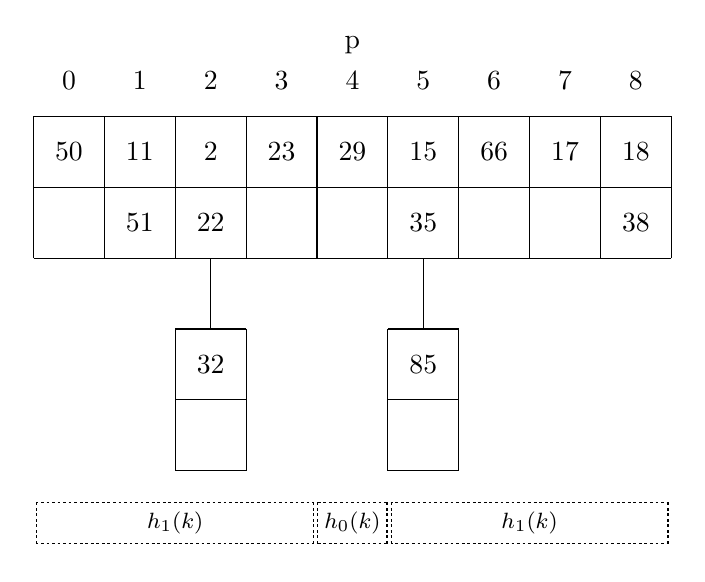
\begin{tikzpicture}
	%template
	\draw[step=.9cm] (1.8, -0.9) grid +(0.9, 1.8);
	\draw[step=.9cm] (4.5, -0.9) grid +(0.9, 1.8);
	\draw[step=.9cm] (0, 1.8) grid +(8.1, 1.8);
	\draw (0, 1.8) -- (8.1, 1.8);
	\draw (1.8, -0.9) -- (1.8, 0.9);
	\draw (2.25, 0.9) -- (2.25, 1.8);
	\draw (4.5, -0.9) -- (4.5, 0.9);
	\draw (4.95, 0.9) -- (4.95, 1.8);
	\draw (1.8, -0.9) -- (2.7, -0.9);
	\draw (4.5, -0.9) -- (5.4, -0.9);
	%index
	\node at (4.05, 4.5) {p};
	\node at (0.45, 4.05) {0};
	\node at (1.35, 4.05) {1};
	\node at (2.25, 4.05) {2};
	\node at (3.15, 4.05) {3};
	\node at (4.05, 4.05) {4};
	\node at (4.95, 4.05) {5};
	\node at (5.85, 4.05) {6};
	\node at (6.75, 4.05) {7};
	\node at (7.65, 4.05) {8};
	%inserted keys
	\node at (0.45, 3.15) {50};
	\node at (1.35, 3.15) {11};
	\node at (1.35, 2.25) {51};
	\node at (2.25, 3.15) {2};
	\node at (2.25, 2.25) {22};
	\node at (2.25, 0.45) {32};

	\node at (3.15, 3.15) {23};
	\node at (4.05, 3.15) {29};
	\node at (4.95, 3.15) {15};
	\node at (4.95, 2.25) {35};
	\node at (4.95, 0.45) {85};
	\node at (5.85, 3.15) {66};
	\node at (6.75, 3.15) {17};
	\node at (7.65, 3.15) {18};
	\node at (7.65, 2.25) {38};
	%hash functions
	\node at (1.8, -1.55) {\dashbox{1}(100,15){\footnotesize $h_1(k)$}};
	\node at (4.05, -1.55) {\dashbox{1}(25,15){\footnotesize $h_0(k)$}};
	\node at (6.3, -1.55) {\dashbox{1}(100,15){\footnotesize $h_1(k)$}};
\end{tikzpicture}

\[\beta = \frac{N}{ (q \cdot 2^{L} + p) \cdot b} = \frac{15}{(5 \cdot 2^{0} + 4) \cdot 2}  = \textcolor{red}{0,83}\]

%10
Splitt von Bucket 4:

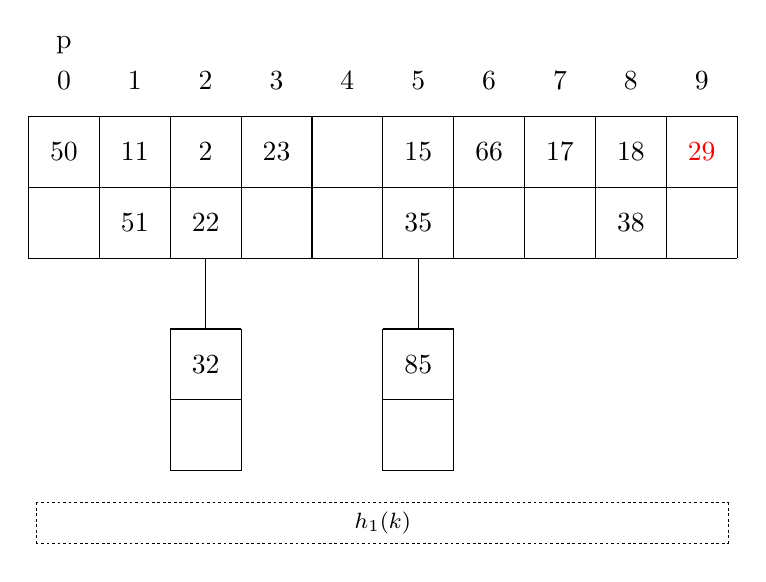
\begin{tikzpicture}
	%template
	\draw[step=.9cm] (1.8, -0.9) grid +(0.9, 1.8);
	\draw[step=.9cm] (4.5, -0.9) grid +(0.9, 1.8);
	\draw[step=.9cm] (0, 1.8) grid +(9, 1.8);
	\draw (0, 1.8) -- (9, 1.8);
	\draw (1.8, -0.9) -- (1.8, 0.9);
	\draw (2.25, 0.9) -- (2.25, 1.8);
	\draw (4.5, -0.9) -- (4.5, 0.9);
	\draw (4.95, 0.9) -- (4.95, 1.8);
	\draw (1.8, -0.9) -- (2.7, -0.9);
	\draw (4.5, -0.9) -- (5.4, -0.9);
	%index
	\node at (0.45, 4.5) {p};
	\node at (0.45, 4.05) {0};
	\node at (1.35, 4.05) {1};
	\node at (2.25, 4.05) {2};
	\node at (3.15, 4.05) {3};
	\node at (4.05, 4.05) {4};
	\node at (4.95, 4.05) {5};
	\node at (5.85, 4.05) {6};
	\node at (6.75, 4.05) {7};
	\node at (7.65, 4.05) {8};
	\node at (8.55, 4.05) {9};
	%inserted keys
	\node at (0.45, 3.15) {50};
	\node at (1.35, 3.15) {11};
	\node at (1.35, 2.25) {51};
	\node at (2.25, 3.15) {2};
	\node at (2.25, 2.25) {22};
	\node at (2.25, 0.45) {32};
	\node at (3.15, 3.15) {23};
	\node at (4.95, 3.15) {15};
	\node at (4.95, 2.25) {35};
	\node at (4.95, 0.45) {85};
	\node at (5.85, 3.15) {66};
	\node at (6.75, 3.15) {17};
	\node at (7.65, 3.15) {18};
	\node at (7.65, 2.25) {38};
	\node at (8.55, 3.15) {\textcolor{red}{29}};
	%hash functions
	\node at (4.5, -1.55) {\dashbox{1}(250,15){\footnotesize $h_1(k)$}};

\end{tikzpicture}

\[\beta = \frac{N}{ (q \cdot 2^{L} + p) \cdot b} = \frac{15}{(5 \cdot 2^{1} + 0) \cdot 2} = 0,75\]

%11
Einfügen der Schlüssel 16 und 59 lässt $\beta > \alpha$ werden:

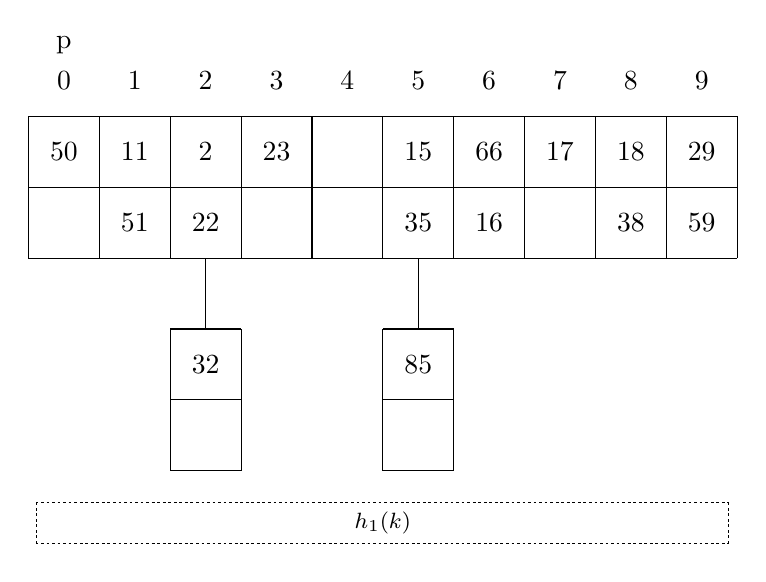
\begin{tikzpicture}
	%template
	\draw[step=.9cm] (1.8, -0.9) grid +(0.9, 1.8);
	\draw[step=.9cm] (4.5, -0.9) grid +(0.9, 1.8);
	\draw[step=.9cm] (0, 1.8) grid +(9, 1.8);
	\draw (0, 1.8) -- (9, 1.8);
	\draw (1.8, -0.9) -- (1.8, 0.9);
	\draw (2.25, 0.9) -- (2.25, 1.8);
	\draw (4.5, -0.9) -- (4.5, 0.9);
	\draw (4.95, 0.9) -- (4.95, 1.8);
	\draw (1.8, -0.9) -- (2.7, -0.9);
	\draw (4.5, -0.9) -- (5.4, -0.9);
	%index
	\node at (0.45, 4.5) {p};
	\node at (0.45, 4.05) {0};
	\node at (1.35, 4.05) {1};
	\node at (2.25, 4.05) {2};
	\node at (3.15, 4.05) {3};
	\node at (4.05, 4.05) {4};
	\node at (4.95, 4.05) {5};
	\node at (5.85, 4.05) {6};
	\node at (6.75, 4.05) {7};
	\node at (7.65, 4.05) {8};
	\node at (8.55, 4.05) {9};
	%inserted keys
	\node at (0.45, 3.15) {50};
	\node at (1.35, 3.15) {11};
	\node at (1.35, 2.25) {51};
	\node at (2.25, 3.15) {2};
	\node at (2.25, 2.25) {22};
	\node at (2.25, 0.45) {32};
	\node at (3.15, 3.15) {23};
	\node at (4.95, 3.15) {15};
	\node at (4.95, 2.25) {35};
	\node at (4.95, 0.45) {85};
	\node at (5.85, 3.15) {66};
	\node at (5.85, 2.25) {16};
	\node at (6.75, 3.15) {17};
	\node at (7.65, 3.15) {18};
	\node at (7.65, 2.25) {38};
	\node at (8.55, 3.15) {29};
	\node at (8.55, 2.25) {59};
	%hash functions
	\node at (4.5, -1.55) {\dashbox{1}(250,15){\footnotesize $h_1(k)$}};

\end{tikzpicture}

\[\beta = \frac{N}{ (q \cdot 2^{L} + p) \cdot b} = \frac{17}{(5 \cdot 2^{1} + 0) \cdot 2} = \textcolor{red}{0,85}\]

%12
Splitt von Bucket 0, $h_2(k)$ kommt hinzu:

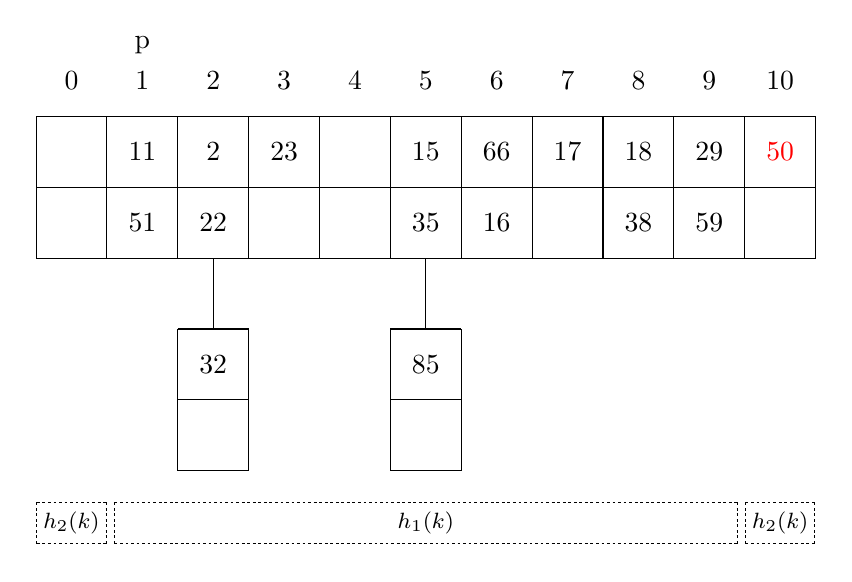
\begin{tikzpicture}
	%template
	\draw[step=.9cm] (1.8, -0.9) grid +(0.9, 1.8);
	\draw[step=.9cm] (4.5, -0.9) grid +(0.9, 1.8);
	\draw[step=.9cm] (0, 1.8) grid +(9.9, 1.8);
	\draw (0, 1.8) -- (9.9, 1.8);
	\draw (1.8, -0.9) -- (1.8, 0.9);
	\draw (2.25, 0.9) -- (2.25, 1.8);
	\draw (4.5, -0.9) -- (4.5, 0.9);
	\draw (4.95, 0.9) -- (4.95, 1.8);
	\draw (1.8, -0.9) -- (2.7, -0.9);
	\draw (4.5, -0.9) -- (5.4, -0.9);
	%index
	\node at (1.35, 4.5) {p};
	\node at (0.45, 4.05) {0};
	\node at (1.35, 4.05) {1};
	\node at (2.25, 4.05) {2};
	\node at (3.15, 4.05) {3};
	\node at (4.05, 4.05) {4};
	\node at (4.95, 4.05) {5};
	\node at (5.85, 4.05) {6};
	\node at (6.75, 4.05) {7};
	\node at (7.65, 4.05) {8};
	\node at (8.55, 4.05) {9};
	\node at (9.45, 4.05) {10};
	%inserted keys
	\node at (1.35, 3.15) {11};
	\node at (1.35, 2.25) {51};
	\node at (2.25, 3.15) {2};
	\node at (2.25, 2.25) {22};
	\node at (2.25, 0.45) {32};
	\node at (3.15, 3.15) {23};
	\node at (4.95, 3.15) {15};
	\node at (4.95, 2.25) {35};
	\node at (4.95, 0.45) {85};
	\node at (5.85, 3.15) {66};
	\node at (5.85, 2.25) {16};
	\node at (6.75, 3.15) {17};
	\node at (7.65, 3.15) {18};
	\node at (7.65, 2.25) {38};
	\node at (8.55, 3.15) {29};
	\node at (8.55, 2.25) {59};
	\node at (9.45, 3.15) {\textcolor{red}{50}};
	%hash functions
	\node at (0.45, -1.55) {\dashbox{1}(25,15){\footnotesize $h_2(k)$}};
	\node at (4.95, -1.55) {\dashbox{1}(225,15){\footnotesize $h_1(k)$}};
	\node at (9.45, -1.55) {\dashbox{1}(25,15){\footnotesize $h_2(k)$}};
\end{tikzpicture}

\[\beta = \frac{N}{ (q \cdot 2^{L} + p) \cdot b} = \frac{17}{(5 \cdot 2^{1} + 1) \cdot 2} = 0,77\]

%13
Einfügen des Schlüssels 9 lässt $\beta > \alpha$ werden:

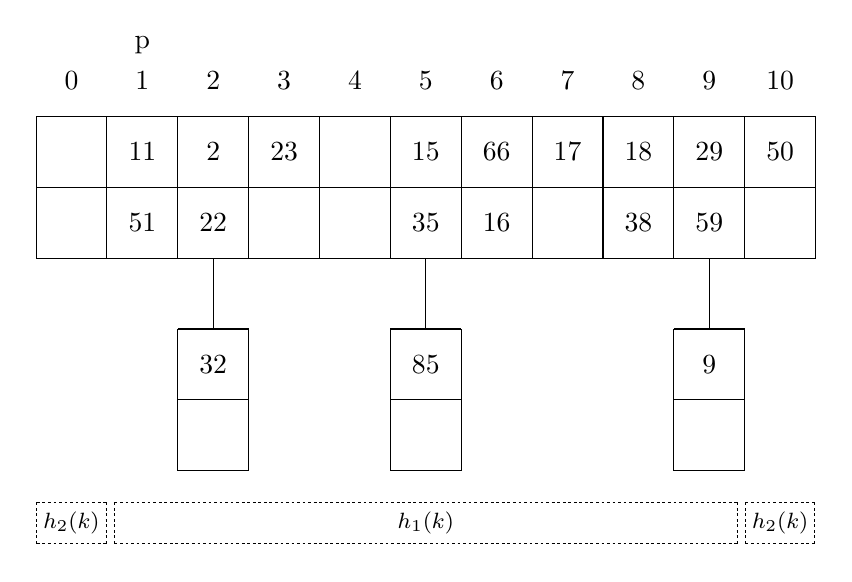
\begin{tikzpicture}
	\def\p{1}
	\def\size{10}
	%template
	\draw[step=.9cm] (1.8, -0.9) grid +(0.9, 1.8);
	\draw[step=.9cm] (4.5, -0.9) grid +(0.9, 1.8);
	\draw[step=.9cm] (8.1, -0.9) grid +(0.9, 1.8);
	\draw[step=.9cm] (0, 1.8) grid +(9.9, 1.8);
	\draw (0, 1.8) -- (9.9, 1.8);
	\draw (1.8, -0.9) -- (1.8, 0.9);
	\draw (2.25, 0.9) -- (2.25, 1.8);
	\draw (4.5, -0.9) -- (4.5, 0.9);
	\draw (4.95, 0.9) -- (4.95, 1.8);
	\draw (8.1, -0.9) -- (8.1, 0.9);
	\draw (8.55, 0.9) -- (8.55, 1.8);
	\draw (1.8, -0.9) -- (2.7, -0.9);
	\draw (4.5, -0.9) -- (5.4, -0.9);
	\draw (8.1, -0.9) -- (9.0, -0.9);
	%index
	\node at (0.45+0.9*\p, 4.5) {p};
	\foreach \i in {0,...,\size}{
		\node at (0.45+0.9*\i, 4.05) {\i};
	}
	\node at (1.35, 3.15) {11};
	\node at (1.35, 2.25) {51};
	\node at (2.25, 3.15) {2};
	\node at (2.25, 2.25) {22};
	\node at (2.25, 0.45) {32};
	\node at (3.15, 3.15) {23};
	\node at (4.95, 3.15) {15};
	\node at (4.95, 2.25) {35};
	\node at (4.95, 0.45) {85};
	\node at (5.85, 3.15) {66};
	\node at (5.85, 2.25) {16};
	\node at (6.75, 3.15) {17};
	\node at (7.65, 3.15) {18};
	\node at (7.65, 2.25) {38};
	\node at (8.55, 3.15) {29};
	\node at (8.55, 2.25) {59};
	\node at (8.55, 0.45) {9};
	\node at (9.45, 3.15) {50};
	%hash functions
	\node at (0.45, -1.55) {\dashbox{1}(25,15){\footnotesize $h_2(k)$}};
	\node at (4.95, -1.55) {\dashbox{1}(225,15){\footnotesize $h_1(k)$}};
	\node at (9.45, -1.55) {\dashbox{1}(25,15){\footnotesize $h_2(k)$}};
\end{tikzpicture}

\[\beta = \frac{N}{ (q \cdot 2^{L} + p) \cdot b} = \frac{18}{(5 \cdot 2^{1} + 1) \cdot 2} = \textcolor{red}{0,82}\]

%14
Splitt von Bucket 1:

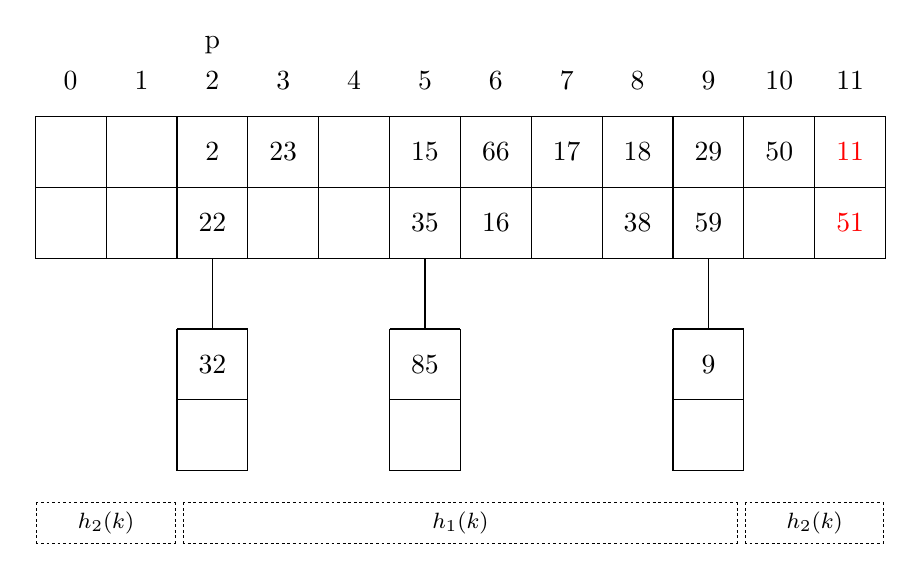
\begin{tikzpicture}
	\def\p{2}
	\def\size{11}
	%template
	\draw[step=.9cm] (1.8, -0.9) grid +(0.9, 1.8);
	\draw[step=.9cm] (4.5, -0.9) grid +(0.9, 1.8);
	\draw[step=.9cm] (8.1, -0.9) grid +(0.9, 1.8);
	\draw[step=.9cm] (0, 1.8) grid +(10.8, 1.8);
	\draw (0, 1.8) -- (10.8, 1.8);
	\draw (1.8, -0.9) -- (1.8, 0.9);
	\draw (2.25, 0.9) -- (2.25, 1.8);
	\draw (4.5, -0.9) -- (4.5, 0.9);
	\draw (4.95, 0.9) -- (4.95, 1.8);
	\draw (8.1, -0.9) -- (8.1, 0.9);
	\draw (8.55, 0.9) -- (8.55, 1.8);
	\draw (1.8, -0.9) -- (2.7, -0.9);
	\draw (4.5, -0.9) -- (5.4, -0.9);
	\draw (8.1, -0.9) -- (9.0, -0.9);
	%index
	\node at (0.45+0.9*\p, 4.5) {p};
	\foreach \i in {0,...,\size}{
		\node at (0.45+0.9*\i, 4.05) {\i};
	}
	%inserted keys
	\node at (2.25, 3.15) {2};
	\node at (2.25, 2.25) {22};
	\node at (2.25, 0.45) {32};
	\node at (3.15, 3.15) {23};
	\node at (4.95, 3.15) {15};
	\node at (4.95, 2.25) {35};
	\node at (4.95, 0.45) {85};
	\node at (5.85, 3.15) {66};
	\node at (5.85, 2.25) {16};
	\node at (6.75, 3.15) {17};
	\node at (7.65, 3.15) {18};
	\node at (7.65, 2.25) {38};
	\node at (8.55, 3.15) {29};
	\node at (8.55, 2.25) {59};
	\node at (8.55, 0.45) {9};
	\node at (9.45, 3.15) {50};
	\node at (10.35, 3.15) {\textcolor{red}{11}};
	\node at (10.35, 2.25) {\textcolor{red}{51}};
	%hash functions
	\node at (0.9, -1.55) {\dashbox{1}(50,15){\footnotesize $h_2(k)$}};
	\node at (5.4, -1.55) {\dashbox{1}(200,15){\footnotesize $h_1(k)$}};
	\node at (9.9, -1.55) {\dashbox{1}(50,15){\footnotesize $h_2(k)$}};
\end{tikzpicture}

\[\beta = \frac{N}{ (q \cdot 2^{L} + p) \cdot b} = \frac{18}{(5 \cdot 2^{1} + 2) \cdot 2} = 0,75\]
\end{solution}
